\documentclass[11pt,a4paper]{article}
\usepackage[margin=0.82in]{geometry}
\usepackage[T1]{fontenc}
\usepackage[utf8]{inputenc}
\usepackage{lmodern}
\usepackage{microtype}
\usepackage{booktabs}
\usepackage{array}
\usepackage{graphicx}
\usepackage{hyperref}
\usepackage{parskip}
\usepackage{titlesec}
\hypersetup{colorlinks=true,linkcolor=black,citecolor=black,urlcolor=blue}
\titlespacing*{\section}{0pt}{0.55em}{0.25em}
\titlespacing*{\subsection}{0pt}{0.45em}{0.15em}
\titleformat{\section}{\normalsize\bfseries}{}{0pt}{}
\titleformat{\subsection}{\small\bfseries}{}{0pt}{}
\setlength{\parskip}{0.32em}
\setlength{\parindent}{0pt}
\setlength{\tabcolsep}{4.5pt}
\renewcommand{\arraystretch}{1.06}

\begin{document}
\begin{center}
{\normalsize\bfseries Essentials in Text and Speech Processing -- Final Report\par}
{\Large\bfseries Robustness of Multilingual Intent Classification to Typos\par}
{\small Ke Sun \qquad Thi Tho Pham \qquad Tristan Hein\par}
\end{center}
\vspace{0.1cm}

\begin{abstract}
We study how controlled character-level corruption affects multilingual intent classification and whether training-time augmentation improves robustness. Using MASSIVE 1.1, we evaluate English, German, Vietnamese, and Simplified Chinese with word and character TF--IDF + Logistic Regression and XLM-R-base. We first run a fixed-setting experiment and then a limited validation-based hyperparameter search over Logistic Regression $C$ and XLM-R learning rate. Models are evaluated on clean input and on deletion, substitution, duplication, and adjacent-swap corruptions at three nominal noise levels. Character features are substantially more robust than word features, while clean-trained XLM-R achieves the best clean performance but loses much of this advantage under corruption. After tuning, mixed-trained XLM-R remains the strongest robust system, with 82.59 clean and 74.75 noisy macro-F1. Our conclusions apply to controlled synthetic character corruption rather than validated natural human typos.
\end{abstract}

\section*{1. Research question and motivation}
Intent classifiers in virtual assistants must map short user utterances to one of many actions, yet real user input is rarely perfectly clean. Even small spelling or typing errors can damage tokenization or lexical matching and change a prediction. Previous work has shown that realistic noise can substantially reduce intent-classification performance and that data augmentation can improve robustness \cite{sengupta2021robustness}. We ask how robust multilingual intent classifiers are to controlled character-level corruption, how robustness differs across representations and languages, and how much typo-augmented training can recover.

The comparison separates three perspectives: a word-level lexical baseline, a character-level representation expected to tolerate local edits better, and a strong multilingual Transformer. We also test whether robustness improves when corrupted examples are included during training.

\section*{2. Data processing and corruption pipeline}
% TEAMMATE CHECK (Thi Tho): verify this concise description against the final data-processing notebook.
We use MASSIVE 1.1 \cite{fitzgerald2023massive,massive_dataset}, a multilingual NLU dataset with 60 intent classes, and select English (\texttt{en-US}), German (\texttt{de-DE}), Vietnamese (\texttt{vi-VN}), and Simplified Chinese (\texttt{zh-CN}). The original splits are cleaned upstream before training: exact training duplicates are removed, normalized-text overlap is checked using Unicode NFKC normalization, case folding and whitespace collapse, the test split is kept unchanged, and overlapping validation/training rows are removed in that order. The retained test split has 2,974 examples per language.

For robustness evaluation, clean utterances are transformed with four controlled character operations: deletion, substitution, duplication, and adjacent-character swapping. Each is generated at nominal noise levels 0.05, 0.10, and 0.20, giving 12 corrupted test conditions per language. Fixed seeds make the exported corruptions reproducible and identical across models. Mixed training contains every clean training example once plus one corrupted copy, so it is a 50/50 clean/corrupted mixture by row count. Test corruptions are never used for training.

These perturbations are \textbf{controlled synthetic character corruptions used as a proxy for typos}. They do not explicitly model keyboard-neighbor errors, German compound spelling, Vietnamese input-method/diacritic errors, or Chinese IME/homophone confusions. The substitution character pool is language-specific but is collected from retained train, validation, and test text, so it uses held-out characters although not held-out labels.

\section*{3. Models and experimental setup}
% TEAMMATE CHECK (Sun): wording follows the finalized Part 02 guide; verify before submission.
The explicit baseline is \textbf{word TF--IDF + Logistic Regression trained on clean data}. We compare it with \textbf{character TF--IDF + Logistic Regression} and fully fine-tuned \textbf{XLM-R-base} \cite{conneau2020xlmr}. The classical models use scikit-learn \cite{pedregosa2011scikit}. Models are trained separately for each language; there is no joint multilingual fine-tuning experiment. For every model family we compare clean-only and mixed training, and all reported runs use seeds 2028, 2029, and 2030 rather than selecting a best seed.

In the original study, Logistic Regression used $C=1$ and XLM-R used learning rate $2\times10^{-5}$. XLM-R selected its best epoch using clean-validation macro-F1, with at most 30 epochs and patience 10. After inspecting the original results, we added a \textbf{supplementary validation-based grid search}: $C\in\{0.1,1,10\}$ for both TF--IDF models and learning rate $\in\{10^{-5},2\times10^{-5},3\times10^{-5}\}$ for XLM-R. For each language/model pair, one value is selected by mean clean-validation macro-F1 across clean and mixed training and all three seeds, and that value is then shared by both training conditions. Test scores are not used to choose the parameter. This is a limited search rather than exhaustive optimization, and because the original test results had already been viewed, we report it explicitly as supplementary tuning rather than an untouched confirmatory study.

We report accuracy and macro-F1, with macro-F1 as the primary robustness metric. ``Noisy'' macro-F1 first averages the 12 corrupted conditions within each seed and then averages seeds; overall summaries weight the four languages equally. The central robustness quantity is the clean-to-noisy macro-F1 drop. Code and experiment documentation are available at \url{https://github.com/phamttho/EssentialsNLP}.

\section*{4. Results}
\subsection*{4.1 Original and tuned model comparison}
The original fixed-setting study already showed the main robustness pattern: word TF--IDF was brittle, character TF--IDF was much more stable under character corruption, and clean-trained XLM-R achieved the strongest clean score but lost much of its advantage under noise. Mixed training helped every model family, especially XLM-R.

The supplementary search strengthens the classical baselines but does not change that conclusion. All eight language/model TF--IDF selections choose $C=10$. English and Chinese XLM-R select $3\times10^{-5}$, while Vietnamese and German keep $2\times10^{-5}$. Table~\ref{tab:overall} shows the original and selected-parameter results. Tuning raises noisy macro-F1 by 4.73--7.53 points for the TF--IDF systems, whereas XLM-R changes by only $-0.05$ points for clean training and $+0.18$ for mixed training. The selected mixed XLM-R remains strongest overall at 74.75 noisy macro-F1.

\begin{table}[ht]
\centering
\small
\caption{Equal-language-weight macro-F1 (\%). Each cell is clean / mean noisy performance.}
\label{tab:overall}
\begin{tabular}{llcc}
\toprule
Model & Training & Original & Selected parameter \\
\midrule
Word TF--IDF + LR & clean & 69.09 / 50.33 & 75.94 / 55.05 \\
Word TF--IDF + LR & mixed & 70.56 / 53.63 & 75.76 / 58.97 \\
Char TF--IDF + LR & clean & 70.37 / 60.32 & 77.51 / 67.85 \\
Char TF--IDF + LR & mixed & 72.67 / 63.62 & 77.11 / 70.01 \\
XLM-R-base & clean & 82.51 / 63.03 & 82.23 / 62.98 \\
XLM-R-base & mixed & \textbf{82.60 / 74.57} & \textbf{82.59 / 74.75} \\
\bottomrule
\end{tabular}
\end{table}

\begin{figure}[t]
\centering
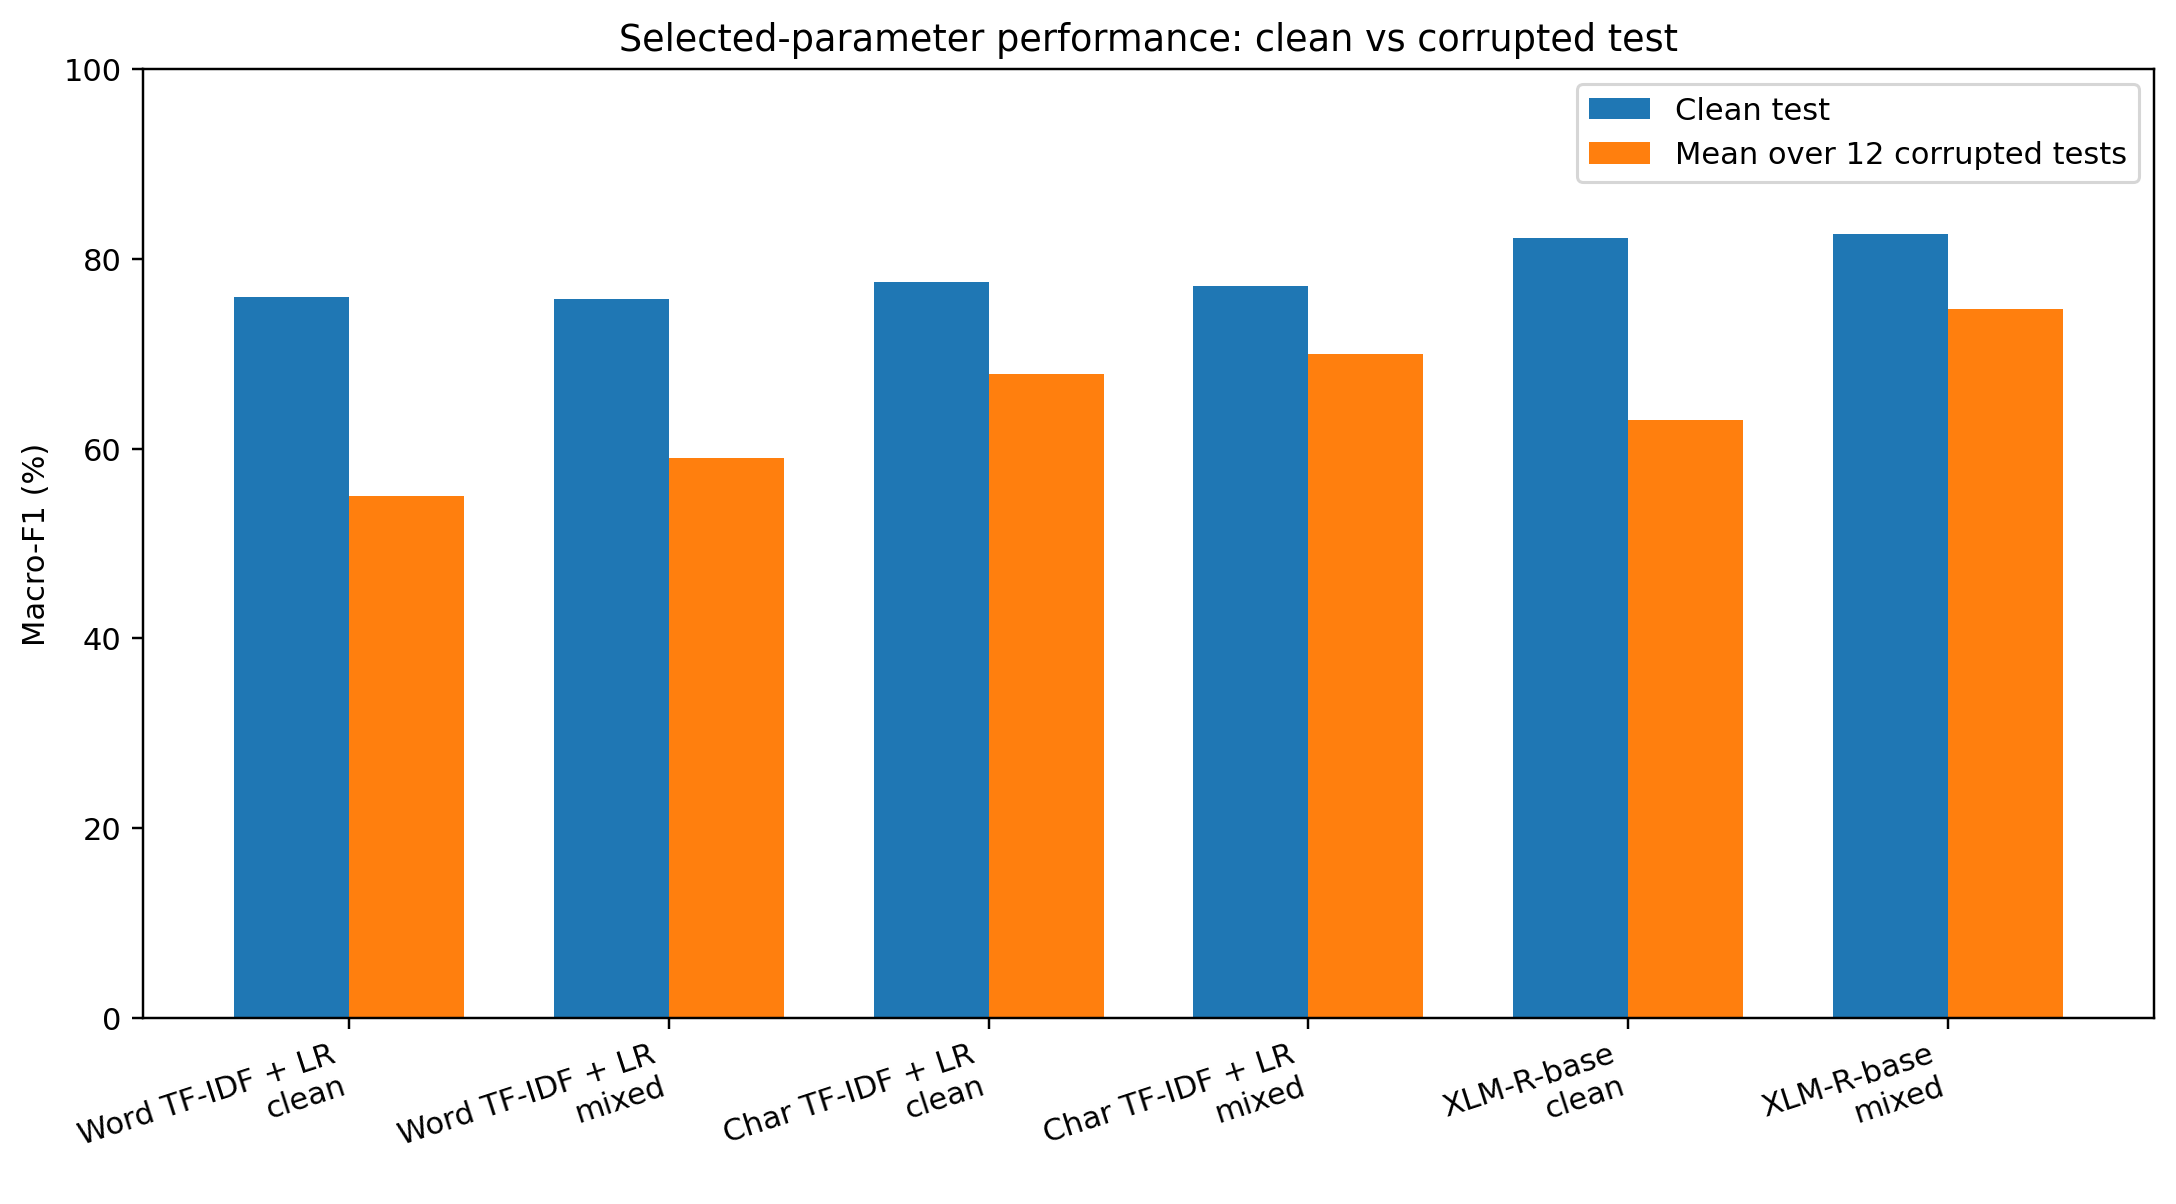
\includegraphics[width=0.92\linewidth]{figures/01_selected_clean_vs_noisy_macro_f1.png}
\caption{Selected-parameter macro-F1 on clean input and the mean over the 12 corrupted test conditions. The figure uses the final HPO three-seed summaries.}
\label{fig:selected-clean-noisy}
\end{figure}

Accuracy tells the same story. With selected parameters, clean/noisy accuracy is 81.34/60.86 for the clean-trained word baseline, 82.52/73.06 for clean-trained character TF--IDF, 86.91/68.12 for clean-trained XLM-R, and 87.02/80.25 for mixed XLM-R. Thus strong clean accuracy alone is not a robustness guarantee.

\subsection*{4.2 Augmentation across languages}
The selected-parameter experiment confirms that augmentation improves average noisy macro-F1 for all 12 language/model pairs, although clean performance can sometimes decrease. For XLM-R, the gain is especially large in English (+17.36 points), German (+13.71), and Vietnamese (+12.25), while Simplified Chinese gains +3.76 points. Table~\ref{tab:xlmr_lang} reports the selected XLM-R mean $\pm$ sample standard deviation across seeds.

\begin{table}[ht]
\centering
\small
\caption{Selected XLM-R macro-F1 (\%), mean $\pm$ SD over three seeds.}
\label{tab:xlmr_lang}
\begin{tabular}{lcc}
\toprule
Language & Clean-trained: clean / noisy & Mixed-trained: clean / noisy \\
\midrule
English & $84.15{\pm}0.44$ / $56.79{\pm}0.17$ & $84.06{\pm}0.46$ / $74.15{\pm}0.60$ \\
Vietnamese & $82.04{\pm}0.04$ / $63.52{\pm}0.65$ & $82.65{\pm}0.37$ / $75.77{\pm}0.25$ \\
German & $81.96{\pm}0.31$ / $57.69{\pm}0.91$ & $82.32{\pm}0.53$ / $71.40{\pm}0.02$ \\
Chinese & $80.76{\pm}0.35$ / $73.93{\pm}0.53$ & $81.32{\pm}0.08$ / $77.69{\pm}0.19$ \\
\bottomrule
\end{tabular}
\end{table}

\begin{figure}[t]
\centering
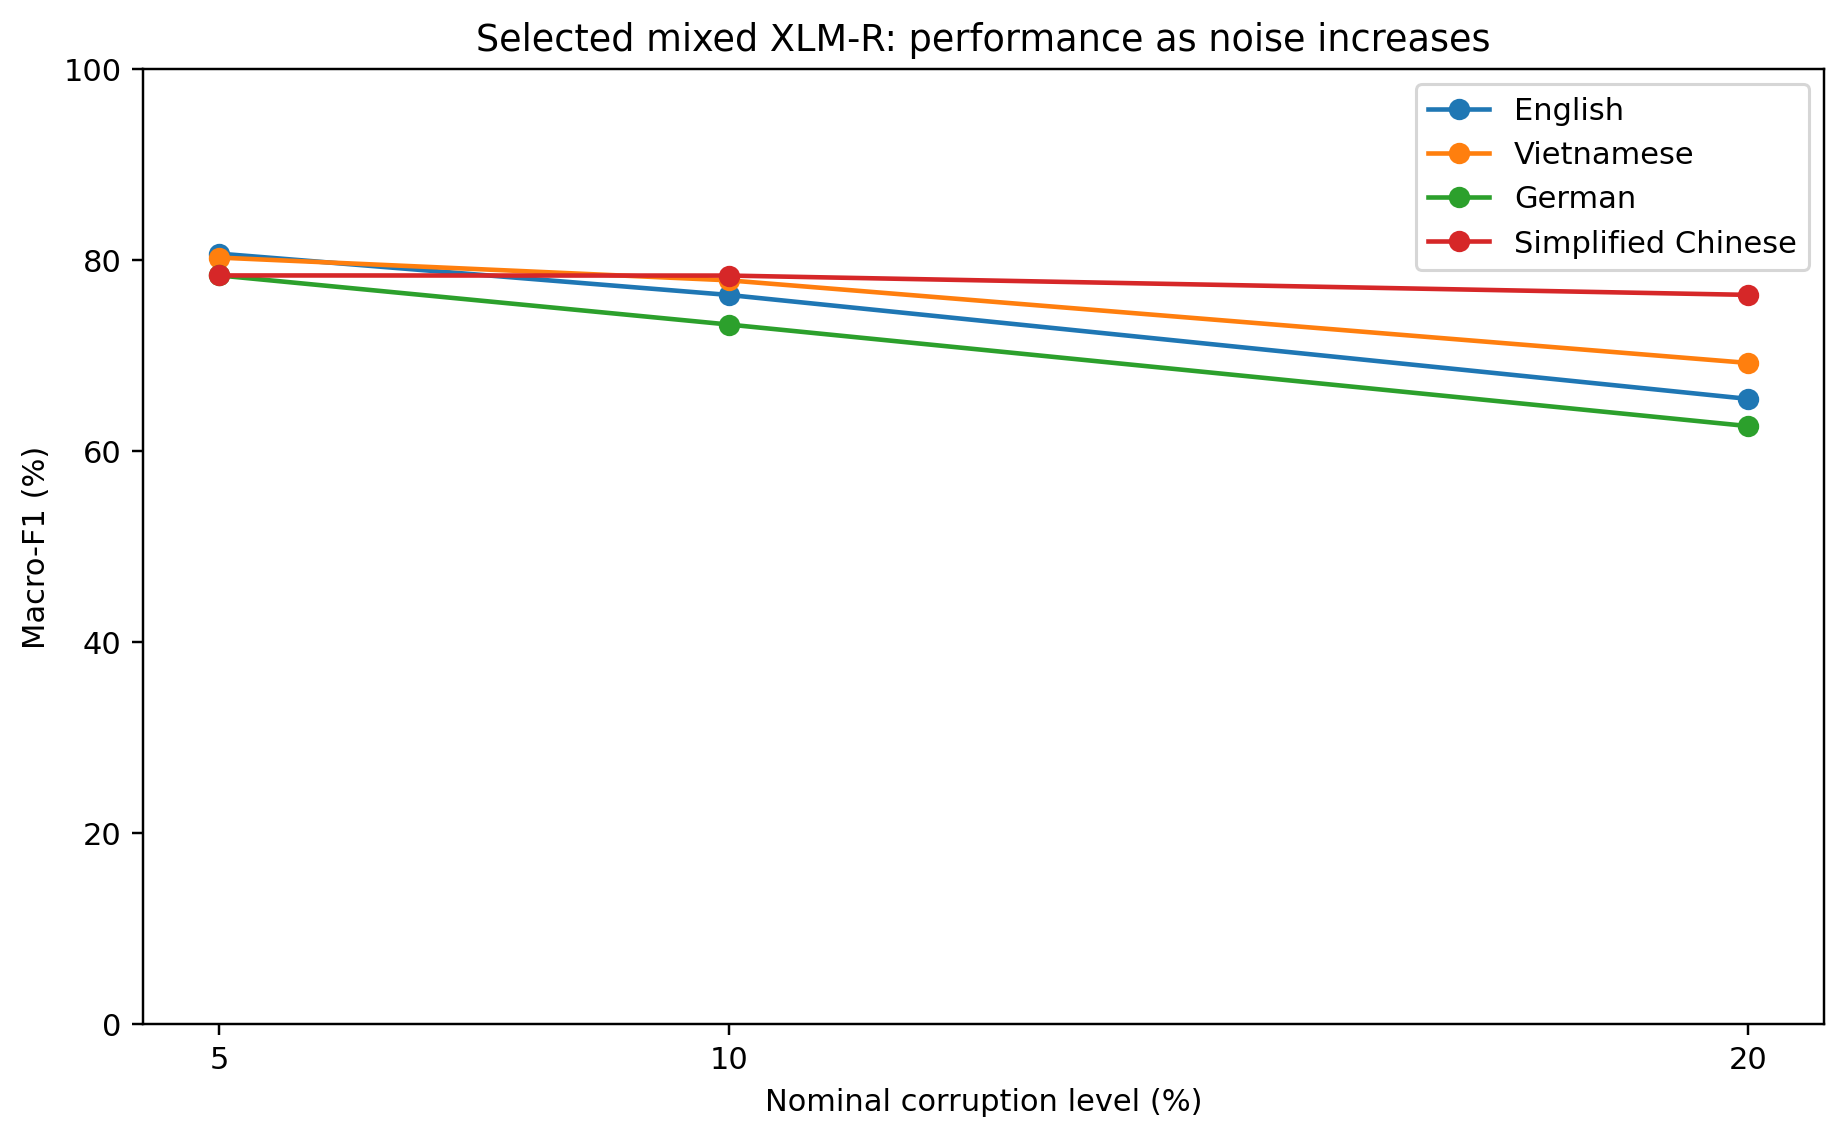
\includegraphics[width=0.78\linewidth]{figures/02_selected_xlmr_noise_curve.png}
\caption{Selected mixed-trained XLM-R macro-F1 as nominal corruption severity increases, averaged over four corruption types and three seeds.}
\label{fig:selected-noise-curve}
\end{figure}

The Chinese XLM-R learning-rate choice is a useful caution: $3\times10^{-5}$ beats $2\times10^{-5}$ on the declared validation criterion by only about 0.009 percentage points, yet slightly reduces noisy test macro-F1 relative to the original setting. Validation-based selection therefore does not guarantee a test improvement, and we keep the declared winner instead of changing it after seeing test results.

\subsection*{4.3 Corruption severity and qualitative errors}
Our detailed corruption-type, severity, confusion, and row-level analyses were performed on the original frozen prediction handoff; the HPO is therefore kept separate from these qualitative results. In the original mixed-XLM-R analysis, performance generally falls as nominal noise increases, and substitution is the most damaging corruption type on average. The same nominal rate should not be treated as identical linguistic difficulty across scripts, so the comparatively small Chinese drop under this synthetic setup is not evidence that Chinese is inherently more robust to real typos.

The corruption audit finds 175 rows marked as corrupted that remain textually unchanged across all generated condition files and six empty outputs produced by deletion. These are a very small share of the evaluation rows but are retained for paired evaluation and reported as a limitation.

Row-level predictions show how local damage changes intent decisions. For example, clean English ``tell me the weather this week'' is correctly classified as \texttt{weather\_query}, while the corrupted ``tell mn uhe weeteer tcis week'' is predicted as \texttt{calendar\_query}. Likewise, ``please remove my alarm'' becomes ``please romzve by alrrm'' and is confused with \texttt{alarm\_set}. Common confusions include \texttt{play\_radio}$\rightarrow$\texttt{play\_music} and \texttt{calendar\_set}$\rightarrow$\texttt{calendar\_query}. Paired examples also show cases where all clean-trained XLM-R seeds fail under corruption while all mixed-trained seeds recover the correct intent, supporting the aggregate augmentation gains.

\section*{5. Discussion and limitations}
Three conclusions are most important. First, \textbf{character-level representations are a strong classical robustness baseline}: after tuning, clean-trained character TF--IDF reaches 67.85 noisy macro-F1 compared with 55.05 for the word baseline. Second, \textbf{clean performance and robustness are distinct}: selected clean-trained XLM-R reaches 82.23 clean macro-F1 but only 62.98 noisy macro-F1, below clean-trained character TF--IDF on noisy input. Third, \textbf{training-time corruption is highly effective for XLM-R}: mixed training raises its selected noisy score from 62.98 to 74.75 while keeping clean performance essentially unchanged (82.23 vs. 82.59).

The supplementary HPO also clarifies what tuning does and does not solve. It substantially improves TF--IDF, but XLM-R changes little overall, and the selected Chinese learning rate slightly worsens test performance. Moreover, all TF--IDF selections lie at the upper tested $C$ boundary, so $C=10$ should not be called a global optimum. The search is intentionally small; n-gram ranges, vocabulary limits, batch size, optimizer, epoch ceiling, and patience are not tuned.

Several limitations remain. The corruptions are synthetic rather than language-specific human errors. Substitution character pools include held-out text characters, swap pairs can overlap, and some corrupted rows are unchanged or empty. The same frozen corruptions are reused for all training seeds, so the reported SD reflects training variability conditional on one corruption realization rather than uncertainty across possible typo samples. Mixed training also doubles the number of examples, so augmentation effects are confounded with additional optimization exposure. We do not run a compute-matched control, significance tests, confidence intervals over regenerated corruptions, or a truncation-rate audit.

For the original fixed-setting handoff, we independently recomputed accuracy and macro-F1 from all 72 saved prediction files. All 936 model/test-condition metric records matched the stored values up to floating-point precision. The supplementary pipeline separately verifies its selected outputs and preserves original versus tuned provenance, reducing the risk that the conclusions result from aggregation or bookkeeping errors.

\section*{6. Conclusion}
Controlled character corruption substantially degrades multilingual intent classification, but the degradation depends strongly on representation and training strategy. Word-level TF--IDF is the most brittle classical baseline, while character TF--IDF is substantially more stable. XLM-R provides the best clean performance but is not automatically robust. Limited validation-based tuning improves the TF--IDF systems considerably but changes XLM-R only slightly, so the original qualitative conclusions remain intact. Mixed typo-augmented XLM-R is the strongest robust system, reaching 74.75 noisy macro-F1 with 82.59 clean macro-F1 after parameter selection.

The practical lesson is that robustness should be evaluated explicitly rather than inferred from clean accuracy, and simple training-time corruption can substantially improve a strong multilingual model. Future work should test whether these findings transfer from controlled synthetic corruption to realistic, language-specific human typing errors and should separate augmentation benefits from the effect of additional training data.

\bibliographystyle{plain}
\bibliography{references}
\end{document}
